

\clearpage
\SourceLeaf{217}%
\begin{center}
[ZUR PARALLELENTHEORIE.]

[\textsc{Schumacher} \emph{an} \textsc{Gauss}.\quad \emph{Copenhagen, 3. Mai 1831.}]
\end{center}

\{\mbox{.\ .\ .\ .\ .\ .\ .\ .} Ich bin so frei Ihnen anbei einen Versuch zu senden, ohne Parallellinien und ihre Theorie zu gebrauchen, den Satz zu beweisen, dass die Summe aller drei Winkel eines geradlinigen Dreiecks $= 180^{0}$ sei, aus dem dann der Beweis des Euklidischen Axioms folgen würde. Ich setze nichts voraus, als dass die Summe aller um einen Punkt liegenden Winkel $= 360^{0} = 4R$, und dass die Wechselwinkel sich gleich sind.

Da ich aus Erfahrung weiss, wie sonderbar blind man (ich wenigstens) mitunter in Bezug auf eigene Arbeiten ist, so fürchte ich sehr, dass eine petitio principii dabei zum Grunde liegt. Ich bin aber jetzt nicht im Stande sie zu entdecken, und erwarte Belehrung von Ihnen.

\textls{[Beilage.]} Man verlängere die Seiten eines geradlinigen Dreiecks $ABC$

\begin{center}
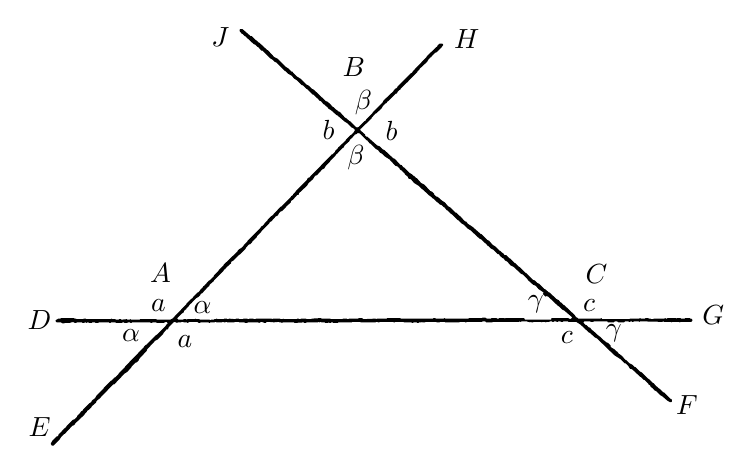
\begin{tikzpicture}[x=0.00683321cm,y=-0.00683321cm]
\fill[even odd rule] (79,811) -- (81,814) -- (84,814) -- (95,803) -- (98,798) -- (104,792) -- (105,792) -- (119,777) -- (122,776) -- (124,774) -- (124,773) -- (142,756) -- (142,755) -- (146,751) -- (146,750) -- (148,748) -- (149,748) -- (155,742) -- (155,741) -- (163,734) -- (164,731) -- (167,728) -- (168,728) -- (195,700) -- (197,700) -- (216,680) -- (221,677) -- (229,668) -- (229,667) -- (236,660) -- (239,659) -- (242,656) -- (243,653) -- (257,638) -- (258,635) -- (273,619) -- (277,617) -- (288,606) -- (288,605) -- (294,598) -- (296,598) -- (297,597) -- (298,594) -- (308,584) -- (312,585) -- (313,586) -- (315,585) -- (321,585) -- (322,584) -- (325,584) -- (326,585) -- (332,585) -- (333,586) -- (337,584) -- (351,584) -- (354,586) -- (356,586) -- (357,585) -- (372,585) -- (374,586) -- (375,585) -- (383,585) -- (384,584) -- (386,584) -- (387,585) -- (397,585) -- (398,584) -- (400,584) -- (401,585) -- (403,585) -- (404,584) -- (406,584) -- (407,585) -- (420,585) -- (421,584) -- (428,584) -- (429,585) -- (439,585) -- (440,586) -- (444,586) -- (445,585) -- (464,585) -- (466,586) -- (470,584) -- (474,585) -- (475,586) -- (478,586) -- (480,584) -- (487,584) -- (488,585) -- (490,584) -- (492,585) -- (503,584) -- (504,585) -- (507,585) -- (508,586) -- (510,585) -- (531,585) -- (532,586) -- (549,585) -- (550,586) -- (553,586) -- (554,585) -- (575,585) -- (576,584) -- (578,585) -- (580,584) -- (582,585) -- (588,585) -- (589,586) -- (594,586) -- (595,585) -- (597,586) -- (599,586) -- (600,585) -- (603,585) -- (604,586) -- (612,586) -- (613,585) -- (638,585) -- (639,584) -- (654,584) -- (655,585) -- (682,585) -- (683,584) -- (686,584) -- (687,585) -- (689,585) -- (690,584) -- (715,584) -- (716,585) -- (718,585) -- (719,584) -- (734,584) -- (735,585) -- (749,585) -- (750,586) -- (752,586) -- (753,585) -- (759,585) -- (760,586) -- (762,586) -- (763,585) -- (767,585) -- (768,584) -- (770,585) -- (774,585) -- (775,584) -- (795,584) -- (796,585) -- (801,585) -- (802,584) -- (811,584) -- (812,585) -- (838,585) -- (839,584) -- (848,584) -- (849,585) -- (851,585) -- (852,584) -- (880,584) -- (881,583) -- (886,583) -- (888,585) -- (899,585) -- (900,584) -- (949,584) -- (950,583) -- (952,584) -- (954,583) -- (964,583) -- (965,584) -- (968,584) -- (969,585) -- (971,584) -- (973,585) -- (975,585) -- (976,584) -- (990,584) -- (991,585) -- (993,584) -- (997,584) -- (999,585) -- (1000,584) -- (1005,584) -- (1006,583) -- (1010,583) -- (1011,584) -- (1013,584) -- (1014,583) -- (1018,583) -- (1019,584) -- (1021,584) -- (1022,583) -- (1026,583) -- (1027,584) -- (1030,584) -- (1031,583) -- (1040,583) -- (1041,584) -- (1055,584) -- (1063,589) -- (1079,604) -- (1080,604) -- (1090,613) -- (1094,615) -- (1126,646) -- (1137,653) -- (1145,661) -- (1147,661) -- (1152,666) -- (1155,671) -- (1159,672) -- (1174,686) -- (1175,686) -- (1181,692) -- (1182,692) -- (1189,699) -- (1189,700) -- (1191,701) -- (1193,703) -- (1193,704) -- (1199,709) -- (1200,711) -- (1204,713) -- (1211,720) -- (1216,723) -- (1224,730) -- (1229,733) -- (1232,733) -- (1233,732) -- (1233,729) -- (1231,727) -- (1230,727) -- (1218,715) -- (1217,715) -- (1210,708) -- (1209,708) -- (1205,704) -- (1204,704) -- (1199,698) -- (1198,698) -- (1190,690) -- (1189,690) -- (1177,678) -- (1173,676) -- (1165,668) -- (1164,668) -- (1160,664) -- (1154,661) -- (1148,655) -- (1147,655) -- (1143,651) -- (1143,650) -- (1136,644) -- (1135,644) -- (1131,639) -- (1130,639) -- (1126,635) -- (1121,632) -- (1119,630) -- (1119,628) -- (1114,623) -- (1111,622) -- (1108,619) -- (1107,619) -- (1099,611) -- (1098,611) -- (1086,600) -- (1085,600) -- (1081,595) -- (1078,594) -- (1074,590) -- (1073,590) -- (1069,586) -- (1069,584) -- (1070,583) -- (1081,583) -- (1082,584) -- (1087,584) -- (1088,583) -- (1113,583) -- (1114,585) -- (1125,585) -- (1127,583) -- (1131,583) -- (1134,585) -- (1144,585) -- (1146,583) -- (1152,583) -- (1153,584) -- (1155,584) -- (1156,583) -- (1158,583) -- (1159,584) -- (1161,584) -- (1162,583) -- (1171,583) -- (1172,584) -- (1174,583) -- (1215,584) -- (1217,583) -- (1218,584) -- (1231,584) -- (1232,585) -- (1234,584) -- (1246,584) -- (1248,585) -- (1249,584) -- (1269,584) -- (1271,582) -- (1271,580) -- (1269,578) -- (1267,578) -- (1266,577) -- (1258,577) -- (1257,578) -- (1250,578) -- (1249,577) -- (1243,577) -- (1242,578) -- (1240,577) -- (1225,577) -- (1224,578) -- (1222,578) -- (1220,577) -- (1219,578) -- (1199,578) -- (1198,579) -- (1194,579) -- (1193,578) -- (1190,578) -- (1189,577) -- (1184,577) -- (1183,578) -- (1175,578) -- (1174,577) -- (1172,578) -- (1155,578) -- (1154,579) -- (1103,579) -- (1102,577) -- (1100,578) -- (1059,578) -- (1057,576) -- (1056,576) -- (1053,573) -- (1053,572) -- (1033,553) -- (1032,553) -- (1027,548) -- (1026,548) -- (1023,544) -- (1019,542) -- (1005,529) -- (1004,529) -- (997,523) -- (996,523) -- (986,513) -- (983,512) -- (978,507) -- (975,506) -- (962,493) -- (961,493) -- (950,482) -- (949,482) -- (942,475) -- (941,475) -- (932,466) -- (931,466) -- (925,460) -- (922,460) -- (919,456) -- (918,456) -- (914,452) -- (913,452) -- (905,444) -- (900,441) -- (893,433) -- (890,432) -- (879,421) -- (878,421) -- (862,407) -- (854,402) -- (851,398) -- (848,397) -- (839,387) -- (838,387) -- (832,381) -- (831,381) -- (822,372) -- (817,369) -- (811,362) -- (806,359) -- (798,352) -- (795,351) -- (791,347) -- (791,346) -- (787,342) -- (784,341) -- (773,329) -- (767,326) -- (759,317) -- (758,317) -- (754,313) -- (753,313) -- (750,310) -- (745,307) -- (735,297) -- (734,297) -- (731,293) -- (728,292) -- (718,281) -- (715,280) -- (699,265) -- (695,263) -- (690,258) -- (685,256) -- (667,240) -- (665,240) -- (663,238) -- (663,236) -- (654,228) -- (654,226) -- (675,206) -- (675,205) -- (682,197) -- (683,197) -- (693,188) -- (696,183) -- (701,178) -- (702,178) -- (705,174) -- (706,174) -- (720,160) -- (721,160) -- (723,158) -- (723,157) -- (727,153) -- (728,153) -- (729,151) -- (741,139) -- (743,138) -- (743,137) -- (760,120) -- (760,119) -- (764,115) -- (764,114) -- (778,101) -- (781,96) -- (785,92) -- (786,92) -- (787,90) -- (793,84) -- (796,83) -- (806,73) -- (806,72) -- (808,70) -- (808,69) -- (806,67) -- (802,67) -- (800,68) -- (797,71) -- (797,72) -- (777,91) -- (777,92) -- (751,119) -- (751,120) -- (749,122) -- (748,122) -- (723,147) -- (723,148) -- (721,150) -- (720,150) -- (716,154) -- (716,155) -- (697,173) -- (695,177) -- (677,195) -- (677,196) -- (665,208) -- (665,209) -- (663,211) -- (662,211) -- (651,222) -- (648,223) -- (646,222) -- (635,211) -- (634,211) -- (627,205) -- (626,205) -- (616,194) -- (613,193) -- (610,190) -- (609,190) -- (604,185) -- (603,185) -- (597,178) -- (596,178) -- (593,175) -- (590,174) -- (568,153) -- (564,151) -- (558,145) -- (554,143) -- (544,133) -- (536,128) -- (529,121) -- (528,119) -- (526,119) -- (520,113) -- (515,110) -- (500,95) -- (494,92) -- (482,79) -- (481,79) -- (466,65) -- (465,65) -- (461,61) -- (460,61) -- (452,53) -- (450,53) -- (435,40) -- (431,40) -- (430,41) -- (430,44) -- (434,49) -- (435,49) -- (439,53) -- (440,53) -- (456,68) -- (459,69) -- (463,73) -- (464,73) -- (470,80) -- (472,80) -- (486,94) -- (491,97) -- (495,101) -- (498,102) -- (514,118) -- (515,118) -- (520,123) -- (527,127) -- (531,132) -- (536,135) -- (545,144) -- (548,145) -- (554,151) -- (555,151) -- (566,162) -- (567,162) -- (574,169) -- (575,169) -- (578,173) -- (581,174) -- (586,180) -- (587,180) -- (591,184) -- (592,184) -- (595,188) -- (600,191) -- (610,200) -- (611,200) -- (625,212) -- (630,215) -- (638,223) -- (641,224) -- (644,227) -- (644,228) -- (641,233) -- (637,237) -- (636,237) -- (627,246) -- (627,247) -- (613,260) -- (613,261) -- (607,267) -- (607,268) -- (602,273) -- (601,273) -- (559,316) -- (558,316) -- (555,319) -- (555,320) -- (534,341) -- (534,342) -- (529,347) -- (529,348) -- (527,350) -- (526,350) -- (525,352) -- (507,370) -- (506,370) -- (490,387) -- (489,387) -- (482,394) -- (482,395) -- (476,401) -- (476,402) -- (472,406) -- (471,406) -- (469,408) -- (469,409) -- (444,434) -- (444,435) -- (437,442) -- (437,443) -- (434,446) -- (429,449) -- (426,452) -- (426,453) -- (400,478) -- (400,479) -- (391,488) -- (391,489) -- (382,498) -- (382,499) -- (374,507) -- (373,507) -- (364,517) -- (362,518) -- (362,519) -- (356,525) -- (356,526) -- (353,529) -- (352,529) -- (343,538) -- (343,539) -- (341,541) -- (340,541) -- (331,550) -- (331,551) -- (305,578) -- (301,580) -- (276,580) -- (275,579) -- (245,579) -- (244,580) -- (228,580) -- (227,579) -- (225,580) -- (221,580) -- (220,579) -- (210,580) -- (209,579) -- (206,579) -- (205,580) -- (200,580) -- (199,579) -- (193,579) -- (192,578) -- (190,579) -- (145,579) -- (144,578) -- (140,578) -- (139,579) -- (127,579) -- (126,578) -- (123,578) -- (122,577) -- (98,577) -- (97,578) -- (93,578) -- (88,581) -- (88,583) -- (90,585) -- (98,585) -- (101,587) -- (104,587) -- (105,586) -- (115,586) -- (116,585) -- (119,585) -- (120,584) -- (124,586) -- (126,586) -- (127,585) -- (137,585) -- (138,586) -- (141,586) -- (142,585) -- (144,585) -- (145,586) -- (147,585) -- (149,585) -- (150,586) -- (155,586) -- (156,585) -- (161,585) -- (162,586) -- (167,586) -- (168,585) -- (187,585) -- (188,586) -- (190,586) -- (191,585) -- (199,585) -- (200,586) -- (211,586) -- (212,585) -- (215,585) -- (216,586) -- (221,586) -- (222,585) -- (226,585) -- (227,586) -- (229,586) -- (230,585) -- (264,585) -- (265,586) -- (267,586) -- (268,585) -- (275,585) -- (276,586) -- (289,586) -- (290,585) -- (294,584) -- (296,586) -- (296,587) -- (293,590) -- (293,591) -- (276,608) -- (275,608) -- (256,627) -- (255,627) -- (252,630) -- (252,631) -- (217,667) -- (217,668) -- (205,680) -- (205,681) -- (199,687) -- (198,687) -- (192,693) -- (191,693) -- (177,707) -- (177,708) -- (164,721) -- (161,726) -- (159,728) -- (158,728) -- (155,731) -- (155,732) -- (152,735) -- (151,735) -- (139,747) -- (139,748) -- (137,750) -- (136,750) -- (134,752) -- (134,753) -- (128,759) -- (128,760) -- (123,765) -- (120,766) -- (108,778) -- (108,779) -- (105,782) -- (104,782) -- (96,791) -- (94,792) -- (93,795) -- (91,797) -- (90,797) -- (81,806) -- (81,807) -- (79,809) -- cycle
(314,578) -- (314,577) -- (323,568) -- (324,568) -- (326,566) -- (326,564) -- (331,560) -- (331,559) -- (336,554) -- (336,553) -- (340,549) -- (341,549) -- (342,547) -- (349,540) -- (353,538) -- (357,534) -- (357,533) -- (359,531) -- (360,531) -- (371,519) -- (373,518) -- (374,515) -- (382,508) -- (382,507) -- (400,489) -- (400,488) -- (402,486) -- (403,486) -- (404,484) -- (414,475) -- (414,473) -- (416,471) -- (417,471) -- (429,459) -- (430,459) -- (441,448) -- (441,447) -- (447,440) -- (449,440) -- (453,436) -- (453,435) -- (462,426) -- (462,425) -- (470,417) -- (470,416) -- (485,401) -- (485,400) -- (487,398) -- (488,398) -- (497,388) -- (501,386) -- (503,382) -- (506,379) -- (509,378) -- (516,371) -- (516,370) -- (525,362) -- (525,360) -- (527,358) -- (528,358) -- (537,348) -- (539,348) -- (540,347) -- (540,345) -- (555,331) -- (558,326) -- (566,319) -- (569,314) -- (571,312) -- (573,312) -- (583,301) -- (587,299) -- (590,294) -- (598,286) -- (598,285) -- (608,275) -- (608,274) -- (611,271) -- (612,271) -- (613,269) -- (621,261) -- (623,260) -- (625,256) -- (633,249) -- (636,244) -- (638,243) -- (644,236) -- (647,235) -- (649,233) -- (653,234) -- (666,247) -- (667,247) -- (672,253) -- (673,253) -- (683,263) -- (687,265) -- (691,270) -- (695,272) -- (700,277) -- (708,282) -- (719,294) -- (723,295) -- (727,299) -- (727,300) -- (729,302) -- (730,302) -- (737,309) -- (737,310) -- (743,315) -- (743,317) -- (744,318) -- (748,319) -- (754,326) -- (762,331) -- (769,338) -- (770,338) -- (784,351) -- (785,351) -- (789,355) -- (790,355) -- (797,362) -- (798,362) -- (802,366) -- (805,367) -- (809,371) -- (810,371) -- (815,377) -- (816,377) -- (823,384) -- (824,384) -- (835,395) -- (836,395) -- (842,401) -- (847,404) -- (854,411) -- (859,414) -- (875,429) -- (879,431) -- (886,438) -- (887,438) -- (891,443) -- (892,443) -- (897,448) -- (901,450) -- (909,458) -- (911,458) -- (913,460) -- (913,461) -- (919,466) -- (920,466) -- (923,470) -- (927,472) -- (933,479) -- (939,482) -- (953,495) -- (956,496) -- (965,505) -- (965,506) -- (975,515) -- (980,517) -- (985,523) -- (994,529) -- (994,531) -- (993,532) -- (998,537) -- (1000,536) -- (1003,537) -- (1022,555) -- (1023,555) -- (1029,561) -- (1033,563) -- (1047,575) -- (1047,577) -- (1044,579) -- (1040,577) -- (1009,577) -- (1009,579) -- (1008,580) -- (960,580) -- (959,579) -- (959,577) -- (924,577) -- (923,578) -- (921,577) -- (912,577) -- (911,578) -- (908,578) -- (907,577) -- (898,577) -- (897,578) -- (889,578) -- (886,576) -- (881,576) -- (880,577) -- (856,577) -- (855,578) -- (812,578) -- (811,577) -- (809,578) -- (794,578) -- (793,577) -- (790,577) -- (789,578) -- (729,578) -- (728,577) -- (704,577) -- (703,578) -- (685,578) -- (684,579) -- (682,578) -- (660,579) -- (657,577) -- (651,577) -- (650,578) -- (633,578) -- (632,579) -- (630,579) -- (629,578) -- (622,578) -- (621,579) -- (599,579) -- (598,578) -- (582,578) -- (581,577) -- (564,578) -- (563,579) -- (554,579) -- (553,578) -- (544,578) -- (543,579) -- (540,579) -- (539,578) -- (537,578) -- (536,579) -- (512,579) -- (511,578) -- (509,579) -- (506,579) -- (505,578) -- (492,578) -- (491,579) -- (489,578) -- (460,578) -- (459,579) -- (456,579) -- (455,578) -- (448,578) -- (447,579) -- (445,579) -- (444,578) -- (437,578) -- (436,579) -- (429,579) -- (428,578) -- (423,578) -- (422,579) -- (410,578) -- (409,579) -- (407,579) -- (406,578) -- (401,578) -- (400,579) -- (389,579) -- (387,578) -- (386,579) -- (383,579) -- (382,580) -- (377,580) -- (376,581) -- (374,580) -- (356,580) -- (355,579) -- (349,579) -- (348,578) -- (346,579) -- (333,579) -- (332,580) -- (330,579) -- (326,579) -- (325,580) -- (316,580) -- cycle;
\node[inner sep=0pt] at (394,55) {$J$};
\node[inner sep=0pt] at (852,58) {$H$};
\node[inner sep=0pt] at (642,111) {$B$};
\node[inner sep=0pt] at (660,176) {$\beta$};
\node[inner sep=0pt] at (595,228) {$b$};
\node[inner sep=0pt] at (712,229) {$b$};
\node[inner sep=0pt] at (646,278) {$\beta$};
\node[inner sep=0pt] at (283,494) {$A$};
\node[inner sep=0pt] at (1093,496) {$C$};
\node[inner sep=0pt] at (279,554) {$a$};
\node[inner sep=0pt] at (1079,554) {$c$};
\node[inner sep=0pt] at (361,557) {$\alpha$};
\node[inner sep=0pt] at (1310,571) {$G$};
\node[inner sep=0pt] at (58,580) {$D$};
\node[inner sep=0pt] at (228,610) {$\alpha$};
\node[inner sep=0pt] at (1038,614) {$c$};
\node[inner sep=0pt] at (328,620) {$a$};
\node[inner sep=0pt] at (1261,738) {$F$};
\node[inner sep=0pt] at (58,779) {$E$};
\node[inner sep=0pt] at (980,552) {$\gamma$};
\node[inner sep=0pt] at (1125,605) {$\gamma$};
\end{tikzpicture}

\par [Fig. 1.]
\end{center}

\noindent unbestimmt, oder man betrachte ein System von drei geraden Linien in einer
